\chapter{Analyse van de reslutaten}%
\label{ch:analyse}

\section{Nauwkeurigheid MQ-sensoren}
\label{sec:nauwkeurigheid}

\subsection{Ammoniak (NH\textsubscript{3})}
\label{subsec:nh3}


\begin{figure}[h!]
    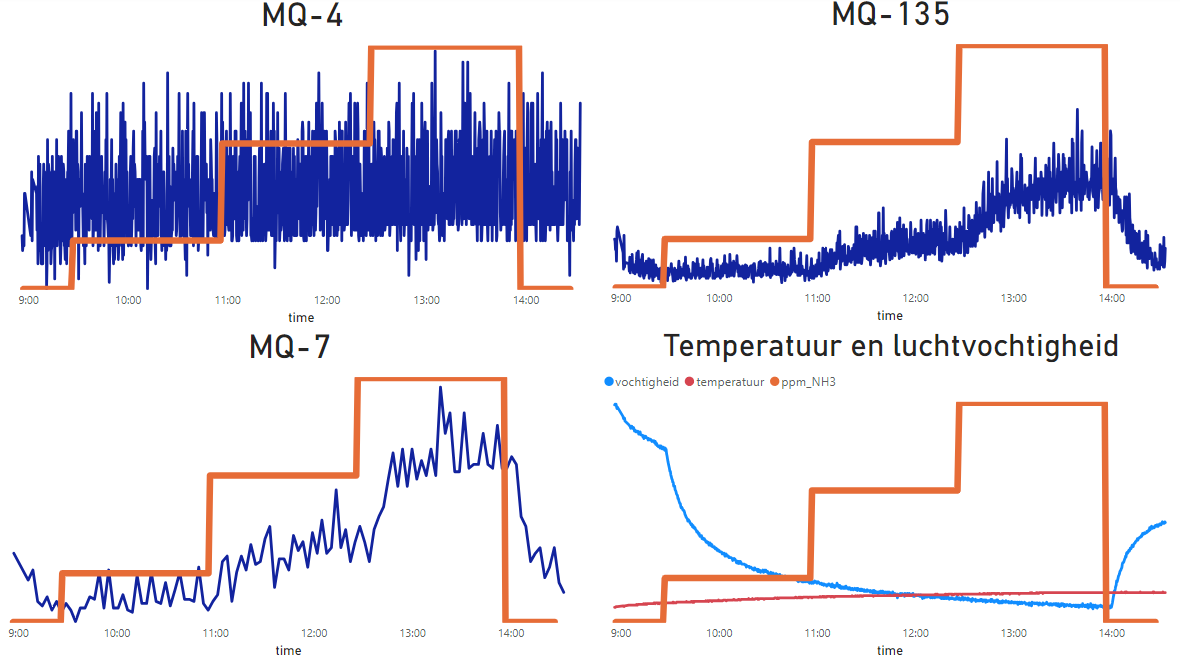
\includegraphics[scale=0.65, center]{NH3_test.png}
    \caption[Test met NH3]{De resultaten van de test met ammoniak}
    \label{fig:NH3_test}
\end{figure}

Figuur~\ref{fig:NH3_test} toont de resultaten van de ammoniak-test. In deze figuur wordt de aangeboden hoeveelheid ammoniak aangetoond door de oranje lijn. Omdat er in de datasheet bij geen van deze 3 sensoren informatie staat over NH\textsubscript{3}, kon dit niet exact worden gemeten. Daarom werd per sensor de gemiddelde waarde berekend van alle gassen. Zo werd vastgesteld dat enkel de MQ-135 en de MQ-7 reageerden op het ammoniakgas. De MQ-4 reageerde helemaal niet.

Ook werd vastgesteld dat de MQ-7 en -135 sensoren moeite hadden met de fase van 1ppm NH\textsubscript{3}, en pas daarna mee begonnen te stijgen. Deze sensoren zullen dus niet gevoelig genoeg zijn om 1 ppm NH\textsubscript{3} te kunnen meten. Zeer verrassend is dit niet, aangezien 1 ppm NH\textsubscript{3} geen hoge hoeveelheid is.

Wat ook zeer duidelijk wordt aan de hand van deze grafieken is dat de drie sensoren elk niet heel stabiel zijn. Naast de vaststelling dat de MQ-7 en -135 sensoren wel degelijk gevoelig zijn voor ammoniak is het moeilijk om hier gefundeerde conclusies uit te trekken.




\subsection{Koolstofdioxide (CO\textsubscript{2})}
\label{subsec:co2}

\begin{figure}[h!]
    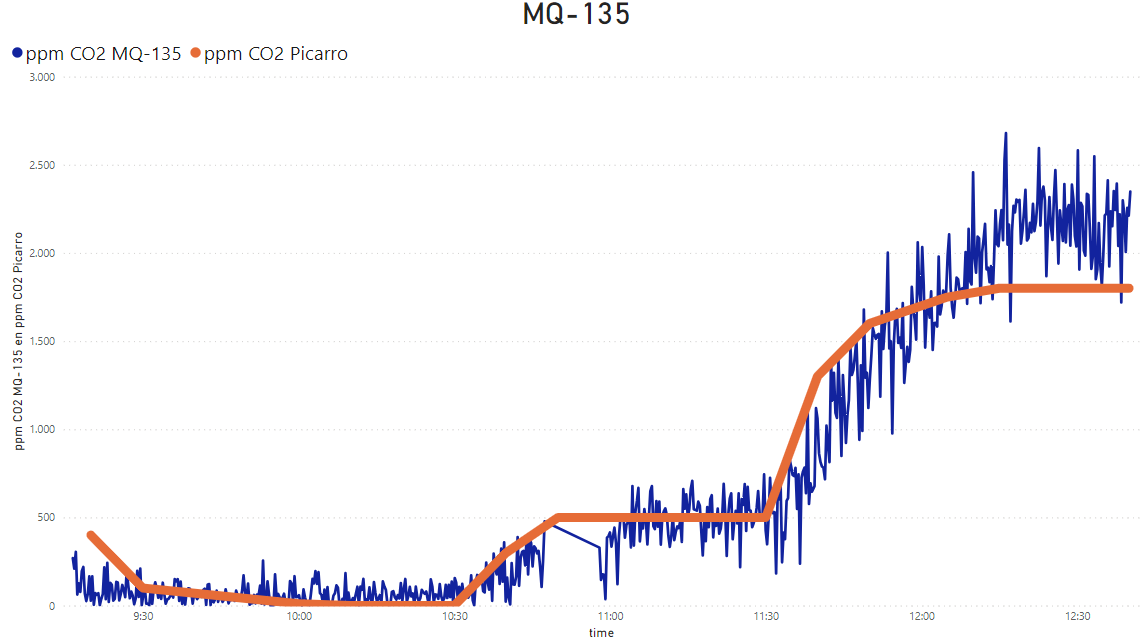
\includegraphics[scale=0.65, center]{CO2_test_135.png}
    \caption[Test met CO2 (MQ135)]{De resultaten van de MQ-135 sensor tijdens de test met CO\textsubscript{2}}
    \label{fig:CO2_test_135}
\end{figure}

Figuur~\ref{fig:CO2_test_135} toont het resultaat van de CO\textsubscript{2} test op de MQ-135 sensor. De referentiewaarde van de Picarro gassensor is aangetoond door de oranje lijn. De blauwe lijn toont de berekende hoeveelheid CO\textsubscript{2} die de MQ-135 heeft gemeten.

In deze grafiek is te zien dat de MQ-135 sensor zeer gevoelig is voor CO\textsubscript{2}. De gemeten ppm CO\textsubscript{2} en de werkelijke hoeveelheid volgen duidelijk dezelfde trend. Ook zijn de gemeten hoeveelheden ppm CO\textsubscript{2} zeer gelijkaardig aan die van de Picarro gassensor. Hiernaast is ook te zien dat de MQ-135 sensor een snelle responstijd heeft, wat een belangrijke factor is bij gassensoren in stalomgevingen.

Echter, ondanks de gevoeligheid en responstijd is de MQ-135 sensor net als in het vorige experiment niet stabiel. Zo valt meteen op dat er zeer veel ruis aanwezig is. Hierdoor is een enkele lezing van de sensor moeilijk betrouwbaar. Ook valt op dat de hoeveelheid ruis toeneemt naarmate er een hogere ppm CO\textsubscript{2} wordt aangeboden.

\pagebreak

\begin{figure}[h!]
    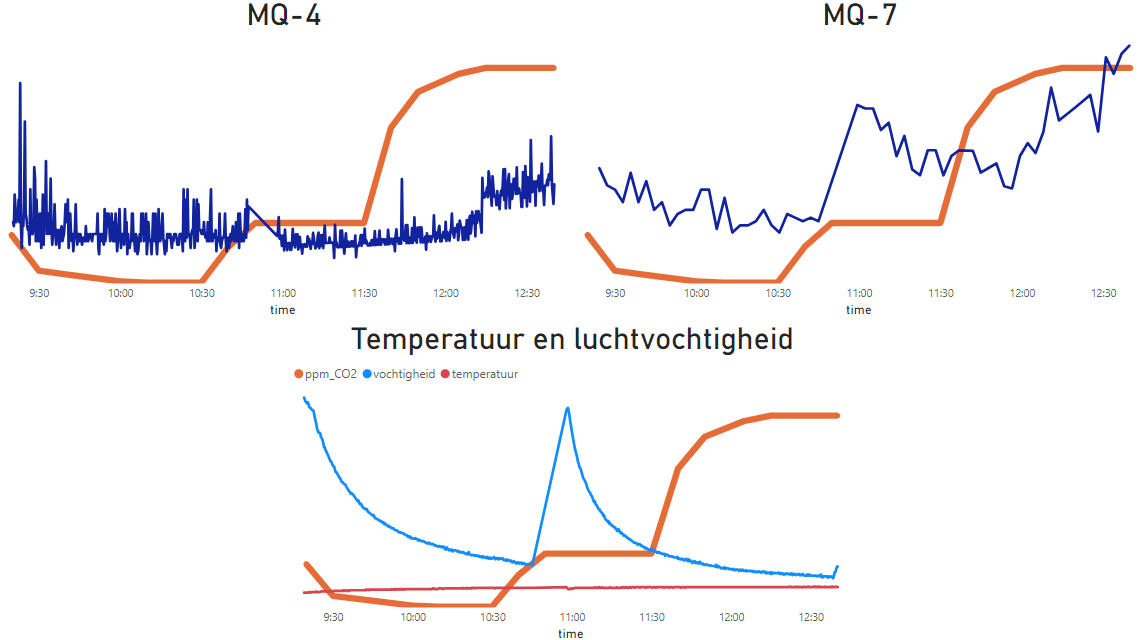
\includegraphics[scale=0.65, center]{CO2_test.png}
    \caption[Test met CO2 (MQ135)]{De resultaten van de MQ-135 sensor tijdens de test met CO\textsubscript{2}}
    \label{fig:CO2_test}
\end{figure}


In figuur~\ref{fig:CO2_test} zijn de resultaten van de andere sensoren te zien. Zo werd voor de MQ-4 en -7 sensor opnieuw een gemiddelde genomen van de waarde aangezien deze niet voorkomt in de datasheets.

In deze figuur is duidelijk te zien dat zowel de MQ-4 als de MQ-7 veel minder gevoelig zijn voor CO\textsubscript{2}. De MQ-4 blijft zeer instabiel en heeft ook veel ruis. In de grafiek is duidelijk te zien dat deze sensor een lage gevoeligheid heeft voor CO\textsubscript{2}. De MQ-7 heeft daarentegen een hogere gevoeligheid dan de MQ-4, maar deze is nog steeds aanzienlijk lager dan de MQ-135 sensor.

Het is belangrijk om op te merken dat er rond 10:45 een storing was waardoor de waarden niet meer werden geüpload naar de databank. Deze is opgelost door de kist te openen. Dit had weinig effect op de hoeveelheid CO\textsubscript{2}, aangezien er op dat moment 500 ppm werd aangeboden, en er ongeveer 400 ppm in de lucht aanwezig is. 

Wel had dit effect op de luchtvochtigheid (\ref{fig:CO2_test}). Waardoor de lezingen van de sensoren in werkelijkheid iets hoger lagen in het volgende kwartier.




\section{Analyse van de warmte-koelcyclus}
\label{sec:analyse_mq7}

Zoals reeds aangehaald in sectie~\ref{sec:warmte_koel} is de warmte-koelcyclus getest in een normale omgeving, dit was buiten, en een omgeving met een hoge luchtvochtigheid, dit was een dampige badkamer. Zo zijn er per omgeving 3 gassen getest: alcohol, CO en LPG. De resultaten werden in de databank opgeslagen en gevisualiseerd in PowerBI. De resultaten zijn te zien op de volgende figuren, waarbij de blootstelling aan het specifieke gas in het rood staat gekleurd.

\begin{figure}[h!]
    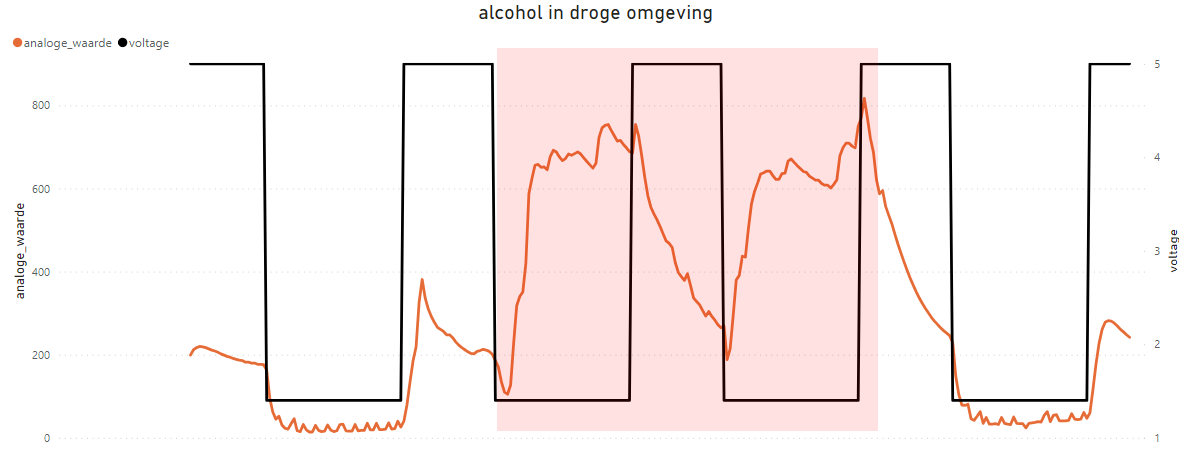
\includegraphics[scale=0.65, center]{alcohol_droog.png}
    \caption[Alcohol in droge omgeving]{Alcohol in droge omgeving}
    \label{fig:alcohol_droog}
\end{figure}

\begin{figure}[h!]
    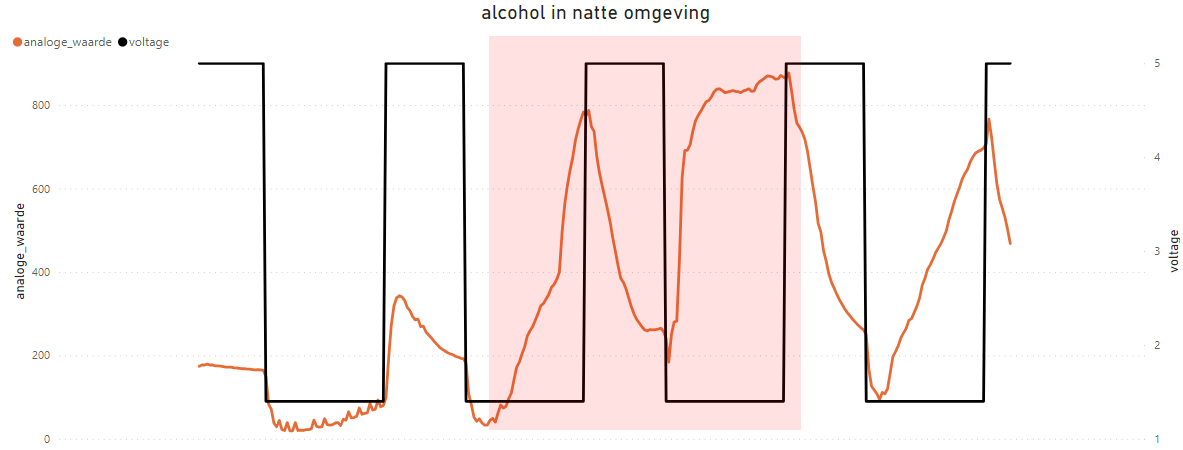
\includegraphics[scale=0.65, center]{alcohol_nat.png}
    \caption[Alcohol in natte omgeving]{Alcohol in natte omgeving}
    \label{fig:alcohol_nat}
\end{figure}

\begin{figure}[h!]
    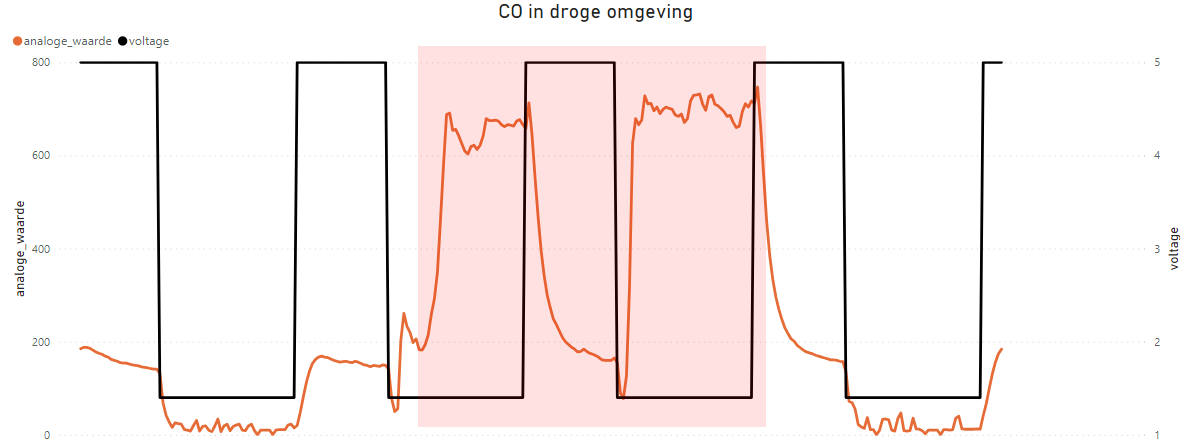
\includegraphics[scale=0.65, center]{co_droog.png}
    \caption[CO in droge omgeving]{CO in droge omgeving}
    \label{fig:co_droog}
\end{figure}

\begin{figure}[h!]
    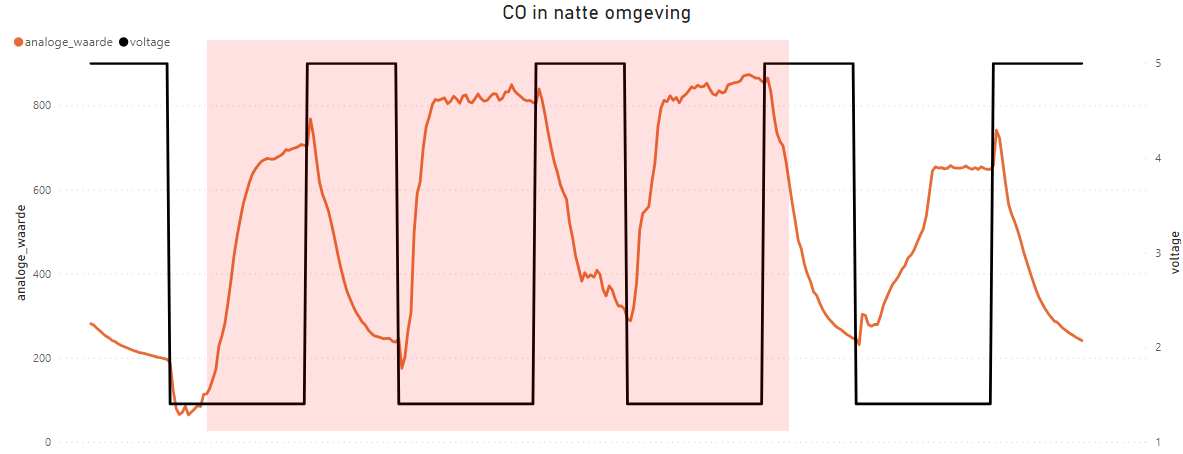
\includegraphics[scale=0.65, center]{co_nat.png}
    \caption[CO in natte omgeving]{CO in natte omgeving}
    \label{fig:co_nat}
\end{figure}

\begin{figure}[h!]
    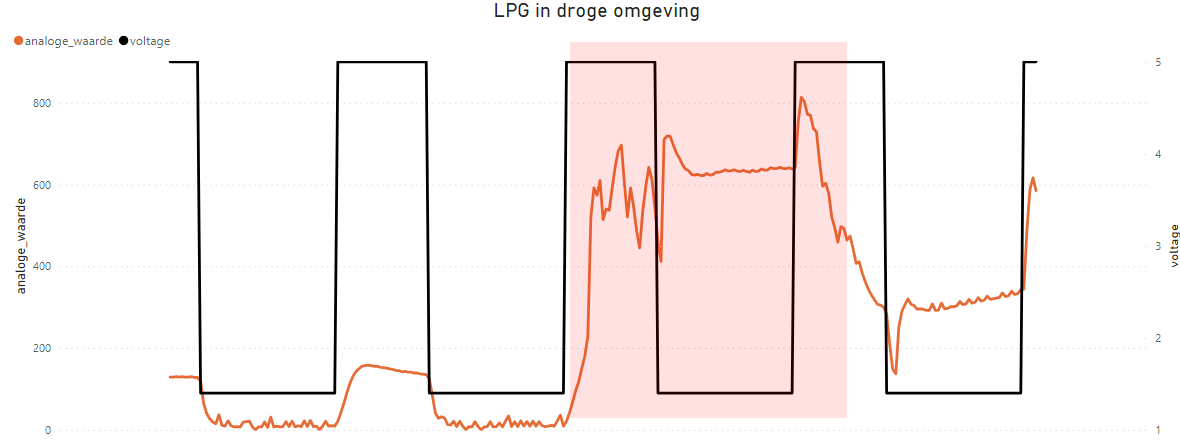
\includegraphics[scale=0.65, center]{lpg_droog.png}
    \caption[LPG in droge omgeving]{LPG in droge omgeving}
    \label{fig:lpg_droog}
\end{figure}

\begin{figure}[h!]
    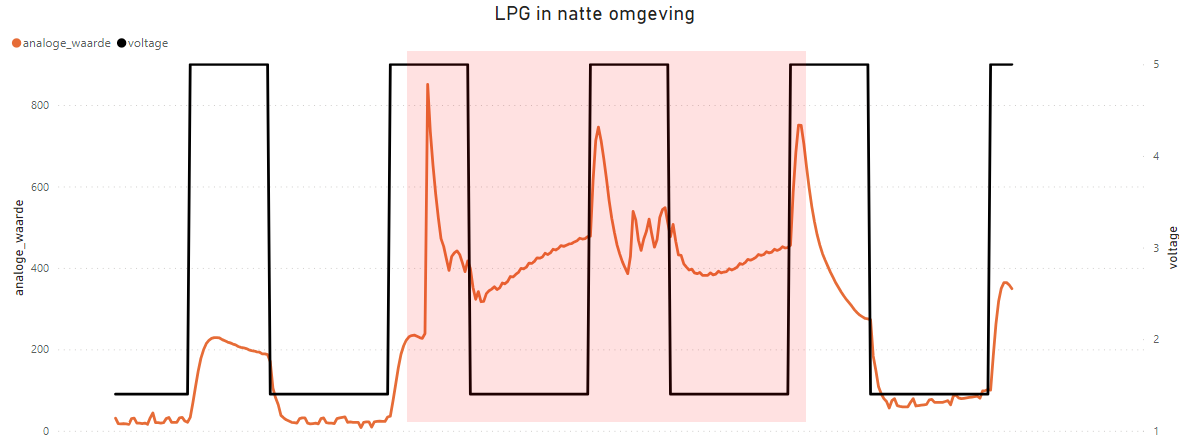
\includegraphics[scale=0.65, center]{lpg_nat.png}
    \caption[LPG in natte omgeving]{LPG in natte omgeving}
    \label{fig:lpg_nat}
\end{figure}


%\pagebreak
\clearpage
\subsection{Invloed van luchtvochtigheid}
\label{subsec:invloed_hum}

Op de resultaten is te zien dat de luchtvochtigheid wel degelijk een rol speelt bij de lezingen van de MQ-7 sensor. 

Het eerste wat opvalt is dat zowel bij alcohol (\ref{fig:alcohol_droog} \&~\ref{fig:alcohol_nat}) als CO (\ref{fig:co_droog} \&~\ref{fig:co_nat}) de waarde hoger is in een vochtige omgeving dan in een normale omgeving, terwijl voor LPG (\ref{fig:lpg_droog} \&~\ref{fig:lpg_nat}) juist het omgekeerde geldt.

Dit verschijnsel kan worden verklaard met het feit dat stoffen homo- en heterogeen kunnen zijn.
Door de vochtige omgeving zit de sensor vol met watermoleculen. Doordat water en LPG sterk heterogeen zijn, en dus net als water en olie niet kunnen worden gemengd, zal deze sensor bij aanraking met LPG een minder hoge waarde uitlezen als normaal. Omdat CO juist homogeen is zijn de waarden hier hoger dan normaal. Bij alcohol kan de mengbaarheid afhangen van het soort alcohol, in dit geval is er ontsmettingsalcohol gebruikt die volgens de deze redenering dus ook homogeen blijkt te zijn met water.

Bij zowel alcohol als CO zijn er weinig verschillen in de droge- en natte grafieken, naast dat de waarde hoger wordt dan normaal en iets stabieler is in de koelfase. Maar bij LPG is er een duidelijker verschil te zien in de koelfase. Zo stabiliseert de waarde vrij snel in de droge omgeving (\ref{fig:lpg_droog}), terwijl ze in natte omgeving (\ref{fig:lpg_nat}) juist heel geleidelijk aan toeneemt.


\subsection{Onderscheiden van verschillende gassen}
\label{subsec:onderscheiding_gassen}


Omdat elk soort gas zich anders gedraagt zouden deze theoretisch gezien onderscheidbaar moeten kunnen zijn op de grafieken. Zo valt meteen de grafiek van CO op (\ref{fig:co_droog}). De MQ-7 sensor is het meest gevoelig voor CO en op de grafiek is dan ook merkbaar hoe snel de waarde klimt wanneer de sensor wordt blootgesteld aan CO. Ook zal de CO het snelste worden weggedreven door een hoge temperatuur.

Alcohol (\ref{fig:alcohol_droog}) klimt daarentegen trager en is veel minder stabiel, waardoor de uiteindelijke lezing na de koelcyclus minder accuraat zal zijn.

LPG heeft ook een merkbare grafiek (\ref{fig:lpg_droog}), zo is te zien hoe LPG zeer stabiel is in de koelcyclus. En tijdens de warmtecyclus een minder grote dip neemt dan de andere gassen. 

Hieruit kan worden opgemerkt dat MQ-7 sensor minder gevoelig is voor alcohol dan LPG en CO. Dit wordt ook aangetoond in de gevoeligheidscurve van de MQ-7 datasheet \autocite{mq7}
te zien in figuur~\ref{fig:MQ7_grafiek}.

\begin{figure}[t]
    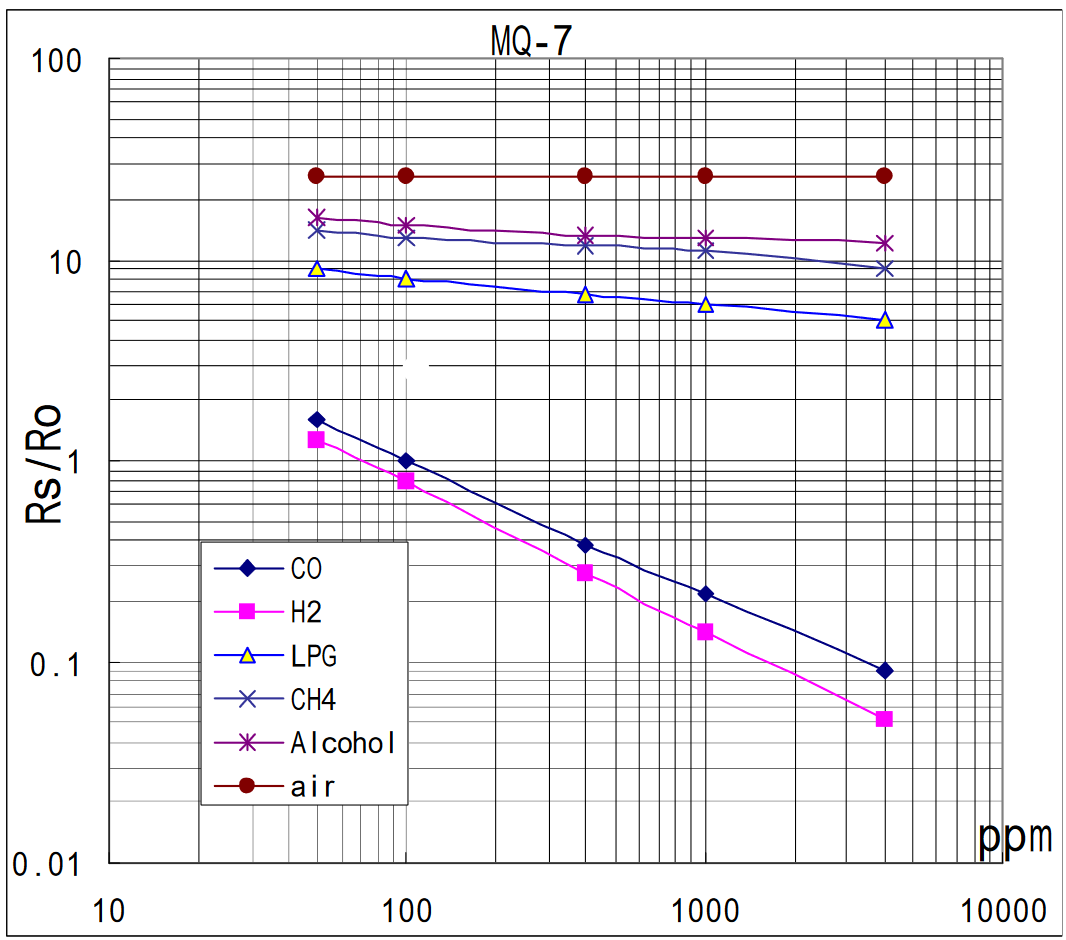
\includegraphics[scale=0.5, center]{MQ7_grafiek.png}
    \caption[Gevoeligheidscurve MQ-7]{Gevoeligheidscurve van de MQ-7 sensor \autocite{mq7}}
    \label{fig:MQ7_grafiek}
\end{figure}













